\section{Unsere Geschäftsidee}
Wir wollen Lösungen für die beschriebenen Probleme des verarbeitenden Gewerbes entwickeln. Durch unseren Predictive-Maintenance-Ansatz kann unser Kunde, der Anlagenbesitzer, in Zukunft proaktiv auf Ereignisse reagieren. Dazu verwenden wir Techniken des maschinellen Lernens aus dem Big-Data-Umfeld. Die individuell für den Kunden ausgewählte Sensorik liefert die benötigten Messdaten für unsere Lösung. 

Unsere Geschäftsidee ist, diese Lösung in Form von IT-Dienstleistung anzubieten. Umsätze generieren neben der Beratungsleistung und der Projektkoordination auch Lizenzerlöse unseres Predictive-Maintenance-Systems.

\subsection{Einflussfaktoren}
\begin{figure}[H]
\centering
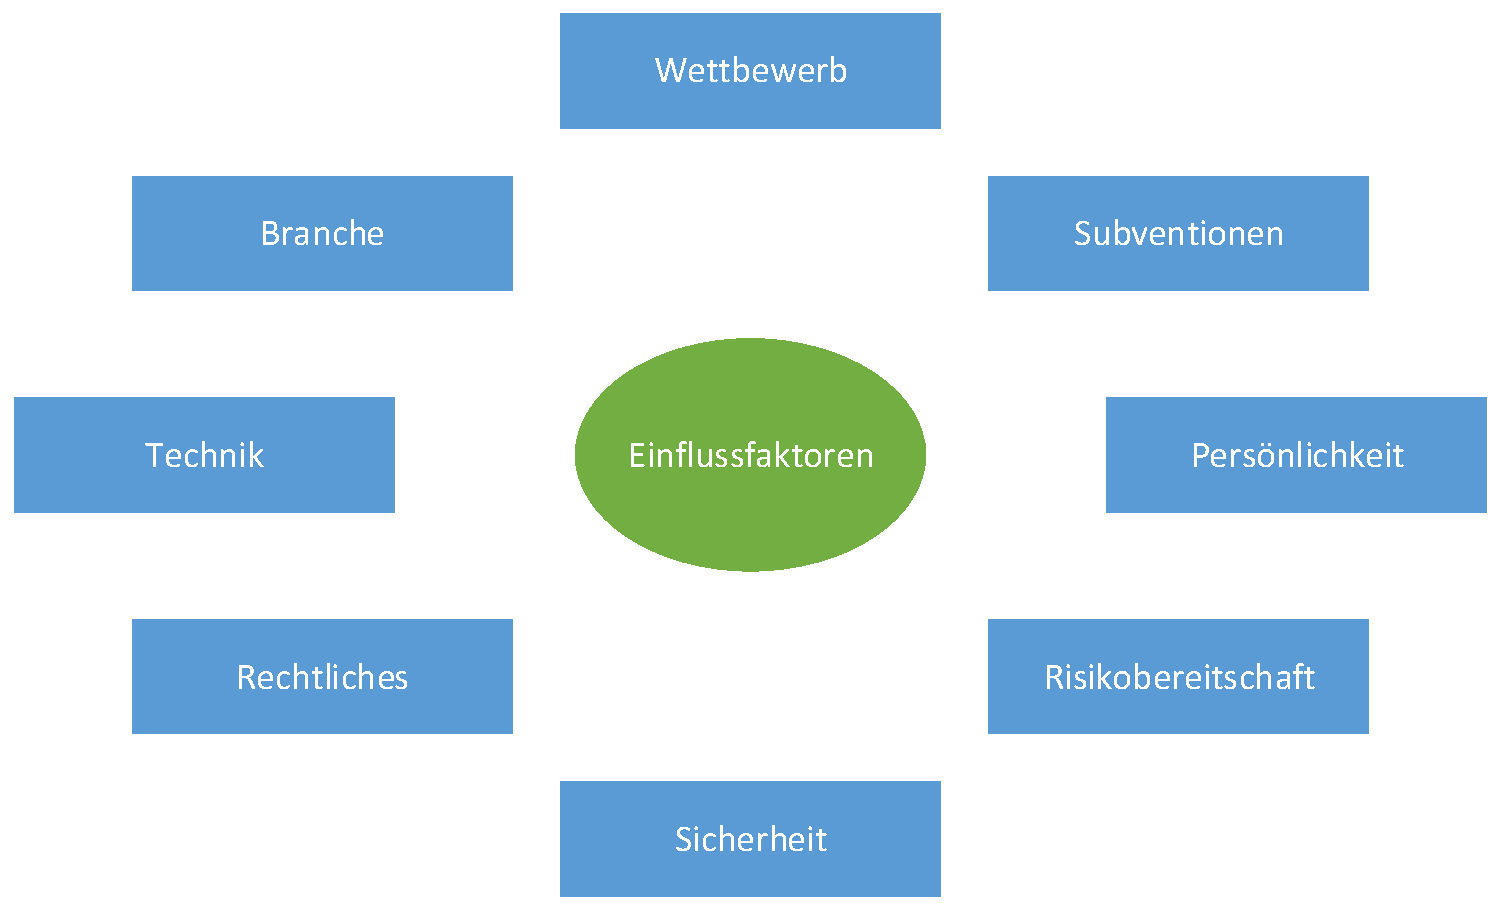
\includegraphics[width=1.0\linewidth]{Bilder/Einflussfaktoren}
\caption{Einflussfaktoren auf unsere Dienstleistung}
\label{fig:Einflussfaktoren}
\end{figure}

\begin{description}
\item[Wettbewerb:]{Der Wettbewerb beschreibt die Marktsituation. Wenn zu viele Wettbewerber in den Markt drängen, macht eine Selbstständigkeit keinen Sinn.}

\item[Subventionen]{Die Bundesregierung subventioniert Industrie 4.0 Anwendungen in ihrer Digitalisierungsoffensive, was unseren potentiellen Kunden den Vorteil verschafft, mit geringerer Eigeninvestition den Sprung in die Zukunft zu schaffen. Für uns bedeutet das eine bessere Auftragslage.}

\item[Persönlichkeit]{Unsere Persönlichkeit stellt einen wichtigen Einflussfaktor auf eine mögliche Selbstständigkeit dar. Bei fehlender Arbeitsbereitschaft und mangelnder Risikobereitschaft ist eine Selbstständigkeit meist von Vornherein zum Scheitern verurteilt.}

\item[Risikobereitschaft]{Die Bereitschaft eines Endkunden das Risiko einzugehen, dass eine Anlage unvorhergesehen ausfällt und die Produktion stoppt, ist für uns äußerst wichtig. Einem Kunden, dem alles egal ist, werden wir keine Predictive-Maintenance-Lösung verkaufen können.}

\item[Sicherheit]{Die Sicherheit von Daten und Anlagen hat höchste Priorität. Eine laufende Produktionsanlage ans Internet anzubinden, muss den höchsten Sicherheitsstandards genügen. Die Möglichkeiten sowie die Bedrohungen in Zukunft stellen einen Einflussfaktor für uns dar.}

\item[Rechtliches]{Die rechtliche Entwicklung im Umgang mit Anlagendaten bzgl. Datenschutz und Verantwortlichkeiten nehmen Einfluss auf unsere Lösungen.}

\item[Technik]{Die aktuell vorhandene sowie zukünftig verfügbare Technik ist einer unserer bedeutendsten Einflussfaktoren. Lösungen für die Verwaltung von Big Data und dessen Auswertung ist ebenso bedeutend wie einsetzbare Sensorik.}

\item[Branche]{Die Branche beeinflusst uns z.B. bei der Standortauswahl oder Ergebnisdefinition in Form von Ofenzuverlässigkeit.}
\end{description}

